\section{Tests}


\subsection{test-1}

El test \texttt{text-1} se encarga de verificar la correctitud de las funciones \mintinline{c++}{void addAndInc(string key)}, \mintinline{c++}{bool member(string key)} y \mintinline{c++}{item maximum(unsigned int nt)}. En él se crea un \texttt{ConcurrentHashMap} y se agregan algunas palabras con \texttt{addAndInc}, verificando luego de cada llamado el valor de \texttt{member}. Para \texttt{maximum} se comprueba su valor usando un solo thread y también usando un cantidad de threads mayor a la cantidad de buckets.


\subsection{test-4}

En el test \texttt{test-4} se prueba la concurrencia de \texttt{addAndInc} creando varios threads que agregan palabras a un mismo \texttt{ConcurrentHashMap}, verificando la pertenencia al map con \texttt{member} y corroborando, una vez que terminan los threads, que \texttt{maximum} devuelve el valor correcto.


\subsection{test-6}

El test \texttt{test-6} tiene el objetivo de poner a prueba la concurrencia de las distintas funciones implementadas. Se crean varios threads que agregan palabras a un mapa propio y a otro mapa compartido por todos, usando distintas cantidades de threads para las funciones concurrentes como \texttt{count\_words} y \texttt{maximum}. La idea es tener una gran cantidad de threads corriendo concurrentemente para tratar de exponer errores. Al final se comprueba si es correcto el valor de \texttt{maximum} de cada uno de los mapas.


\subsection{test-7}

El fin de este test es comparar el tiempo de ejecución de las dos versiones de la función \mintinline{c++}{item maximum(unsigned int p_archivos, unsigned int p_maximos, list<string> archs)}: la que usa un mapa por thread y luego los combina en uno (\texttt{maximum}) y la que llama a \texttt{count\_words} (\texttt{maximum2}).

Se espera que \texttt{maximum} sea más lento que \texttt{maximum2} ya que el primero crea varios mapas que luego debe combinar, mientras que el segundo cuenta las palabras con sólo un mapa.

Para la prueba se ejecutaron las funciones para una lista de mil archivos, usando valores de \texttt{p\_archivos} y \texttt{p\_maximos} de 1 a 5.

En la figura \ref{fig:test_tiempos} se puede ver efectivamente que el tiempo de ejecución de \texttt{maximum} es mayor al de \texttt{maximum2} en todos los casos, llegando a ser más de 50\% más lento.

\begin{figure}[!h]
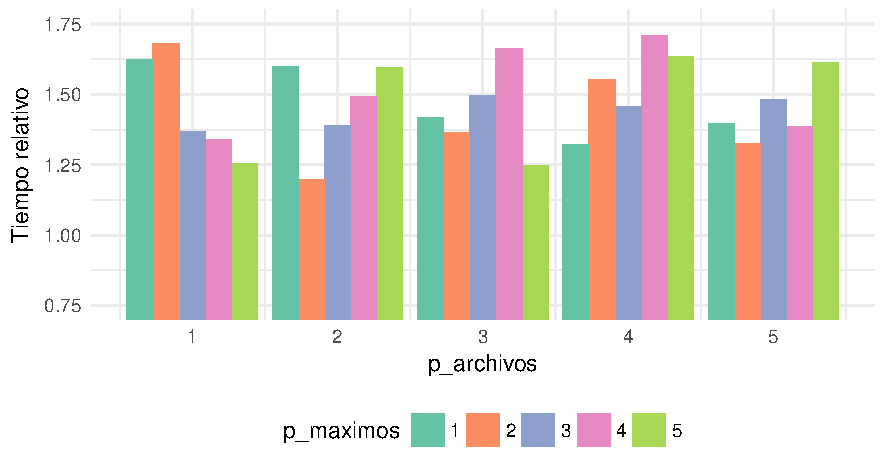
\includegraphics{figuras/tiempos.pdf}
\caption{Tiempo de \texttt{maximum} relativo al tiempo de \texttt{maximum2}}
\label{fig:test_tiempos}
\end{figure}